\documentclass[aspectratio=169]{beamer}

\usepackage{amssymb,amsmath}
\usepackage{graphicx}
\usepackage{url}
\usepackage{color}
\usepackage{pagenote}[continuous,page]
\usepackage{relsize}		% For \smaller
\usepackage{url}			% For \url
\usepackage{epstopdf}	% Included EPS files automatically converted to PDF to include with pdflatex

%For MindMaps
% \usepackage{tikz}%
% \usetikzlibrary{mindmap,trees,arrows}%

%%% Color Definitions %%%%%%%%%%%%%%%%%%%%%%%%%%%%%%%%%%%%%%%%%%%%%%%%%%%%%%%%%
%\definecolor{bordercol}{RGB}{40,40,40}
%\definecolor{headercol1}{RGB}{186,215,230}
%\definecolor{headercol2}{RGB}{80,80,80}
%\definecolor{headerfontcol}{RGB}{0,0,0}
%\definecolor{boxcolor}{RGB}{186,215,230}

%%% Save space in lists. Use this after the opening of the list %%%%%%%%%%%%%%%%
%\newcommand{\compresslist}{
%	\setlength{\itemsep}{1pt}
%	\setlength{\parskip}{0pt}
%	\setlength{\parsep}{0pt}
%}

%\setbeameroption{show notes on top}

% You should run 'pdflatex' TWICE, because of TOC issues.

% Rename this file.  A common temptation for first-time slide makers
% is to name it something like ``my_talk.tex'' or
% ``john_doe_talk.tex'' or even ``discrete_math_seminar_talk.tex''.
% You really won't like any of these titles the second time you give a
% talk.  Try naming your tex file something more descriptive, like
% ``riemann_hypothesis_short_proof_talk.tex''.  Even better (in case
% you recycle 99% of a talk, but still want to change a little, and
% retain copies of each), how about
% ``riemann_hypothesis_short_proof_MIT-Colloquium.2000-01-01.tex''?

\mode<presentation>
{
  \usetheme{CambridgeUS}		% bem bacana - menu superior
  \usecolortheme{default}		% branco, azul clarinho
  \useoutertheme{default}
  \useinnertheme{circles}
  \setbeamercovered{invisible}
}

\beamertemplatenavigationsymbolsempty

%% Better looking blocks
\setbeamercolor{block title alerted}{use=structure,fg=black,bg=red!80!black}
\setbeamercolor{block body alerted}{use=structure,fg=black,bg=white!90!black}

\setbeamercolor{block title}{use=structure,fg=black,bg=blue!60!white}
\setbeamercolor{block body}{use=structure,fg=black,bg=white!90!black}

\usepackage[english]{babel}
\usepackage[latin1]{inputenc}
\usepackage{subfigure}

\usepackage{times}
\usepackage[T1]{fontenc}

%% makes the ppagenote command for figure references at the end.
\makepagenote
\renewcommand{\notenumintext}[1]{}
\newcommand{\ppagenote}[1]{\pagenote[Page \insertframenumber]{#1}}


\title[GB13624]{GB13624 - Maths for Computer Science}
\subtitle[]{Lecture 0 -- About this Course}
\author[Claus Aranha]{Claus Aranha\\{\footnotesize caranha@cs.tsukuba.ac.jp}}
\institute[COINS]{College of Information Science}
\date[]{{\tiny Last updated \today}}

\begin{document}

\section{Introduction}
\subsection{Outline}

\begin{frame}
  \maketitle
\end{frame}

\begin{frame}
  \frametitle{What is this course about?}

  In this course, you will study (or review?) topics in fundamental mathematics that are \structure{useful for computer scientists}.

  \vfill

  \begin{itemize}
  \item Central topic: Discrete Mathematics
    \begin{itemize}
    \item Proofs
    \item Sets
    \item Integers
    \item Combinations
    \item Probability
    \end{itemize}
  \bigskip

  \item Theoretical version of "Programming Challenges"?
  \end{itemize}


  \bigskip

  A \structure{secondary objective} of this lecture is to help you \structure{practice your technical English}.
\end{frame}


\begin{frame}
  \frametitle{Course Materials}


  This course is based on \structure{Mathematics for Computer Science, Spring 2015}, by Albert Meyer and Adam Chlipala, Massachusetts Institute of Technology (MIT), OpenCourseWare (OCW)

  \bigskip

  The original MIT materials, as well as the materials prepared for this   version of the course are licensed as Creative Commons BY-NC-SA.

  \bigskip

  \begin{center}
    
\includegraphics[width=0.2\textwidth]{../img/by-nc-sa}
  \end{center}

  \bigskip

  In \structure{manaba} you can find links to the original course, as well as the textbook.\\
  \alert{Make sure to read the textbook along with this course!}
\end{frame}

\begin{frame}
  \frametitle{Structure of a Lesson}

  \begin{enumerate}
    \item Learn this week's topics;
    \begin{itemize}
      \item Please ask lots of questions in class!
    \end{itemize}
    \item Present the weekly homework;
    \begin{itemize}
      \item Start working on the weekly homework;
      \item You can ask questions about the homework in class;
    \end{itemize}
    \item Submit the homework on manaba
  \end{enumerate}

  \bigskip
  \begin{block}{End time}
    If you have finished the homework, you may leave the class early.
  \end{block}
\end{frame}

% \begin{frame}
%   \frametitle{Structure of a Lesson}
%   \framesubtitle{\structure{Hybrid Online Version}}
%
%   This year, our lecture will be \alert{On-demand Online}. Each week includes the following activities:
%   \bigskip
%
%   \begin{enumerate}
%   \item Watch the video about the week's topic on MS stream;
%   \begin{itemize}
%     \item You can watch the video at any time. Some of the videos are the same as last year.
%   \end{itemize}
%   \item Join the "Office Hours" during the class period, on MS Teams;
%   \begin{itemize}
%     \item During the regular lecture time, the professors will be available on MS teams to answer questions about the materials and the exercise.
%   \end{itemize}
%   \item Solve the weekly exercise;
%   \begin{itemize}
%     \item Every week there is one exercise related to that week's subject. Try to start the exercise during office hours.
%   \end{itemize}
%   \end{enumerate}
%
% \end{frame}

\begin{frame}
  \frametitle{Course Topics}
  \begin{itemize}
  \item Part I: Proofs
    \begin{itemize}
    \item Class 1: Introduction to Proofs
    \item Class 2: Sets and Induction
    \end{itemize}
  \item Part II: Structures
    \begin{itemize}
    \item Class 1: Number Theory
    \item Class 2: Directed Graphs and Partial Orders
    \item Class 3: Simple and Planar Graphs
    \end{itemize}
  \item Part III: Counting
    \begin{itemize}
    \item Class 1: Sums and Assymptotics
    \item Class 2: Cardinality Rules and Generating Functions
    \end{itemize}
  \item Part IV: Probability
    \begin{itemize}
    \item Class 1: Events, Probability Spaces, Conditionals
    \item Class 2: Random Variables, Deviation from Mean, Random Walk
    \item Class 3: Advanced Topics and Review
    \end{itemize}
  \end{itemize}
\end{frame}

% \begin{frame}
%   \frametitle{Course Evaluation}
%   \begin{itemize}
%   \item 50\% Weekly Exercises
%     \begin{itemize}
%     \item One to three questions will be posed in class;
%     \item Students may discuss the answers in class, but the report must be individual;
%     \item Submission must be a PDF on MANABA;
%     \end{itemize}
%
%     \bigskip
%
%   \item 50\% Final Exam
%   \end{itemize}
%
%   \vfill
%
%   \begin{block}{Extra Credit}
%     I often give extra credit to students who participate in class
%     with questions, interesting comments, good suggestions, etc.
%   \end{block}
% \end{frame}

\begin{frame}{Course Evaluation}{\structure{Online Version}}

  The grade of this course will be the weighted average between the Weekly Exercises and the Final Exam.\bigskip

  \begin{itemize}
  \item 70\% Weekly Exercises
    \begin{itemize}
    \item One to three questions will be posed in class;
    \item You must answer your exercises individually;
    \item Submission must be a PDF on MANABA;
    \end{itemize}
    \bigskip

  \item 30\% Final Exam
  \begin{itemize}
    \item The final exam will cover topics from all lectures;
    \item The final exam will probably be \alert{Face to Face}; Let me know if you have problems.
  \end{itemize}
  \end{itemize}
\end{frame}

\begin{frame}
  \frametitle{About the Course Language}

  One of the goals of this lecture is to raise your level of technical
  English. However, this is not an English Class.

  \bigskip

  I expect the students to submit their exercises and exam answers in
  English. It does not need to be perfect, but I expect you to make a
  good effort.

  \bigskip

  \begin{block}{If you are having difficulties}
    Please contact me by MANABA message, MS Teams, or by e-mail at any time!
  \end{block}

\end{frame}

\begin{frame}
  \frametitle{Self-introduction}
  \begin{columns}
    \column{0.4\textwidth}
    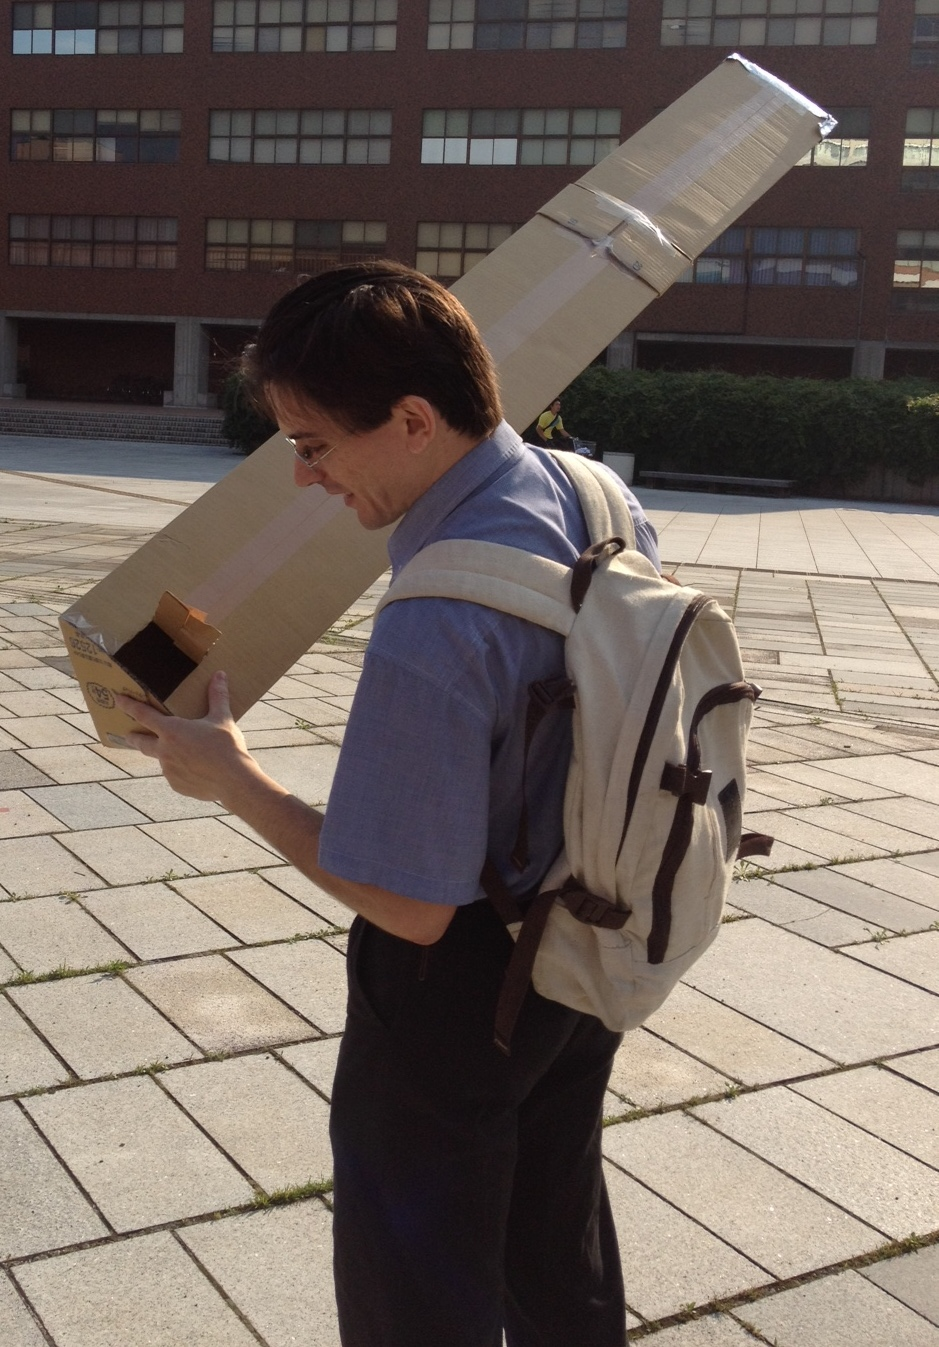
\includegraphics[width=1\textwidth]{../img/pinhole}
    \column{0.6\textwidth}
           {\small
             \begin{itemize}
             \item \structure{Name:} Claus Aranha;
               \medskip

             \item \structure{Country:} Brazil;
               \medskip

             \item \structure{Research:} Evolutionary Computation and Artificial Life;
               \medskip

             \item \structure{Hobby:} game programming
               \medskip

             \item \structure{Webpage:}
               \url{http://conclave.cs.tsukuba.ac.jp}
             \end{itemize}
           }
  \end{columns}
\end{frame}
\end{document}
